\section{Système électrique}

\subsection{Architecture d'alimentation}

Le scanner est alimenté depuis le secteur 230\,V\textsubscript{AC}
(exigence \textbf{E20}) par une alimentation externe qui fournit le bus
principal basse tension. Un convertisseur abaisseur dérive le 5\,V
nécessaire au Raspberry Pi et à l'électronique logique. L'architecture
deux-rails sépare la partie puissance, principalement le moteur et le
laser, de la partie commande.

\begin{figure}[H]
  \centering
  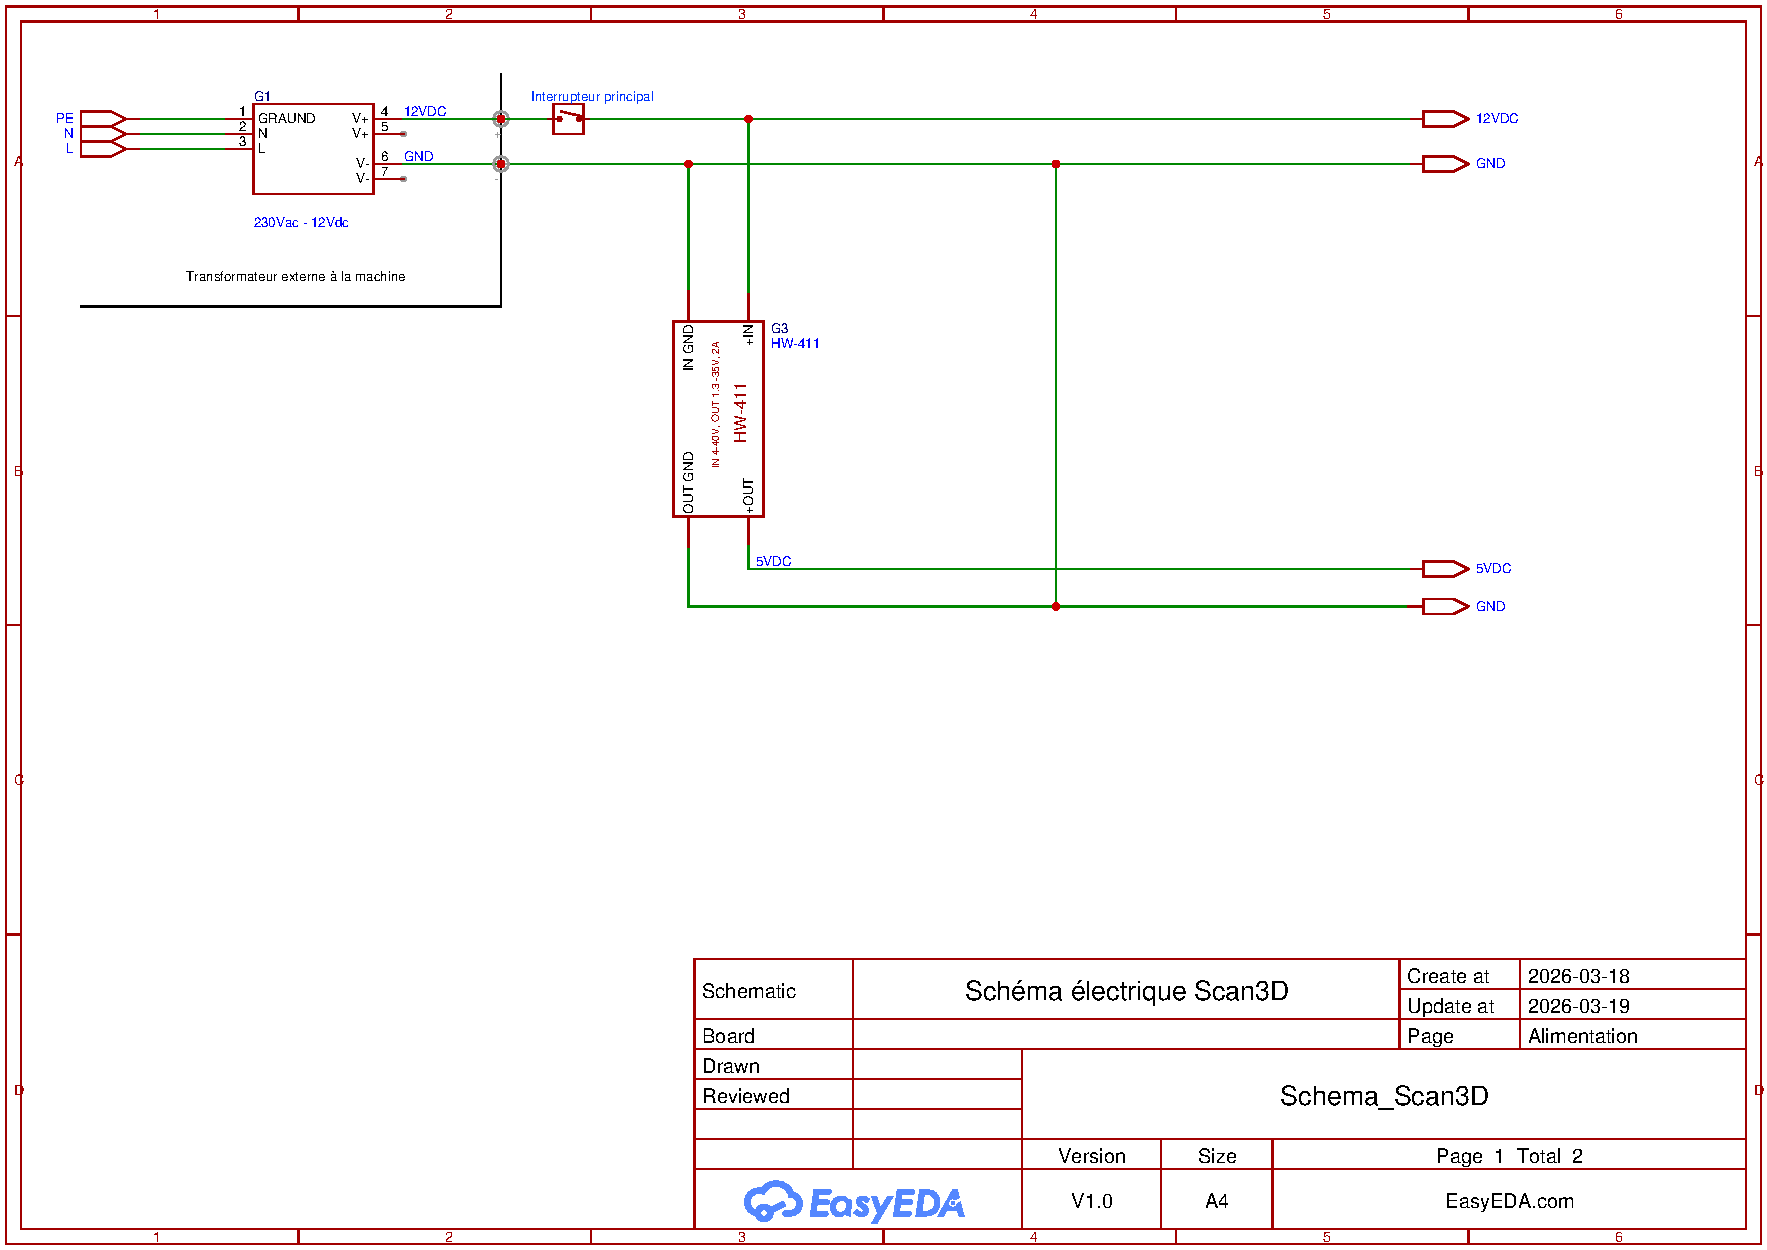
\includegraphics[width=\linewidth,page=1]{assets/Schema_electrique_Scan3D.pdf}
  \caption{Schéma électrique — étage d'alimentation.}
  \label{fig:sch-alim}
\end{figure}

\subsection{Distribution et protection}

\begin{table}[H]
  \centering
  \begin{tabular}{@{}p{3cm}p{3cm}p{7.5cm}@{}}
    \toprule
    \textbf{Rail} & \textbf{Source} & \textbf{Charges} \\
    \midrule
    12\,V\textsubscript{DC} & Alimentation externe & Moteur pas-à-pas via DM320T, laser \\
    5\,V\textsubscript{DC}  & Convertisseur DC/DC & Raspberry Pi 4, écran, logique \\
    3{,}3\,V                & Régulateur interne Pi & GPIO, capteur de porte prévu \\
    GND                     & Commun                & Tous les sous-systèmes \\
    \bottomrule
  \end{tabular}
  \caption{Rails d'alimentation et répartition des charges.}
  \label{tab:rails}
\end{table}

\paragraph{Protection utilisateur.}
Le choix d'une alimentation externe limite la présence de tensions
dangereuses dans la boîte. La partie accessible du prototype fonctionne
en basse tension. La version finale devra toutefois intégrer un câblage
propre, une coupure générale claire et une protection mécanique des
conducteurs.

\paragraph{Sécurité laser.}
La coupure électrique du laser doit rester prioritaire par rapport au
confort d'utilisation. L'interlock de capot, non encore monté pendant les
essais, devra empêcher l'activation du laser lorsque la boîte est ouverte.

\subsection{Bilan de consommation}

Le bilan de consommation reste à mesurer précisément sur le prototype
final. Les valeurs du tableau ci-dessous sont donc des ordres de grandeur
ou des points à caractériser, pas des mesures validées. Les essais actuels
montrent toutefois que l'alimentation choisie permet de faire fonctionner
le Raspberry Pi, la caméra, le laser, le moteur, les LEDs et l'écran
pendant un cycle de scan.

\begin{table}[H]
  \centering
  \begin{tabular}{@{}p{4cm}p{2.5cm}p{2.5cm}p{4.5cm}@{}}
    \toprule
    \textbf{Charge} & \textbf{Tension} & \textbf{Courant à vérifier} & \textbf{Statut} \\
    \midrule
    Raspberry Pi 4      & 5\,V   & À mesurer en charge & Fonctionnel en test \\
    Écran tactile 7 pouces & 5\,V & À mesurer & Fonctionnel en test \\
    Laser ligne         & 5\,V   & À mesurer & Commande fonctionnelle \\
    Moteur NEMA\,17 + DM320T & 12\,V & Dépend du réglage courant driver & Rotation fonctionnelle \\
    Caméra USB prévue   & 5\,V   & À mesurer & À intégrer si retenue \\
    \bottomrule
  \end{tabular}
  \caption{Bilan de consommation intermédiaire.}
  \label{tab:conso}
\end{table}

\subsection{Validation intermédiaire}

Les validations réalisées à ce stade sont fonctionnelles : le système
peut être alimenté, lancer un scan réel, commander le moteur et le laser,
acquérir des images et produire un résultat de reconstruction. Les mesures
électriques détaillées restent à effectuer avant la version finale.

\begin{itemize}
  \item Vérifier que l'alimentation reste stable pendant un scan complet.
  \item Valider la coupure du laser en cas d'erreur et lors de
        l'ouverture du capot.
  \item Confirmer la marge d'alimentation si une deuxième caméra USB est
        ajoutée.
\end{itemize}

\subsection{Limites identifiées et actions prévues}

\begin{itemize}
  \item Finaliser la séquence de mise sous tension pour éviter les états
        transitoires indésirables.
  \item Documenter le câblage final et les connecteurs.
  \item Ajouter la sécurité capot avant tout usage par un utilisateur non
        encadré.
  \item Mesurer la consommation réelle pour confirmer la marge disponible.
\end{itemize}
